\documentclass{beamer}
\usetheme{Warsaw}

\setbeamercolor{normal text}{fg=white,bg=black!90}
\setbeamercolor{structure}{fg=white}

\setbeamercolor{alerted text}{fg=red!85!black}

\setbeamercolor{item projected}{use=item,fg=black,bg=item.fg!35}

\setbeamercolor*{palette primary}{use=structure,fg=structure.fg}
\setbeamercolor*{palette secondary}{use=structure,fg=structure.fg!95!black}
\setbeamercolor*{palette tertiary}{use=structure,fg=structure.fg!90!black}
\setbeamercolor*{palette quaternary}{use=structure,fg=structure.fg!95!black,bg=black!80}

\setbeamercolor*{framesubtitle}{fg=white}

\setbeamercolor*{block title}{parent=structure,bg=black!60}
\setbeamercolor*{block body}{fg=black,bg=black!10}
\setbeamercolor*{block title alerted}{parent=alerted text,bg=black!15}
\setbeamercolor*{block title example}{parent=example text,bg=black!15}

\definecolor{blue}{rgb}{0,0.5,1}

\graphicspath{{figures/}}

\usepackage[ngerman]{babel}

\title{Informatik: Zahlensysteme}
\subtitle{Dezimal- \& Binärsystem}
\author{sca,kng}
\institute{KSR}
\date{\today}

\begin{document}

\begin{frame}
    \titlepage
\end{frame}

\begin{frame}
    \frametitle{Warm-Up I}
    Uhrzeit 1:
    \begin{figure}[H]
        \centering
        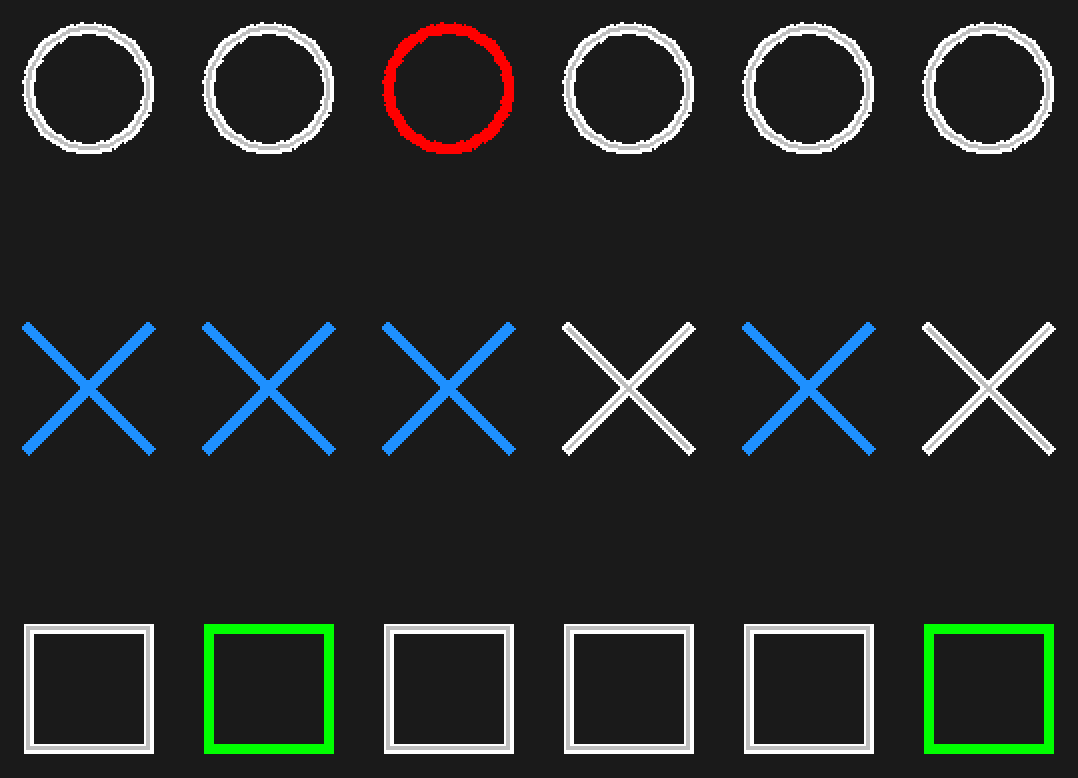
\includegraphics[width=0.7\textwidth]{08_58_17_dark}
    \end{figure}
    \onslide<2-> $$08:58:17$$
\end{frame}

\begin{frame}
    \frametitle{Warm-Up I}
    \begin{figure}[H]
        \centering
        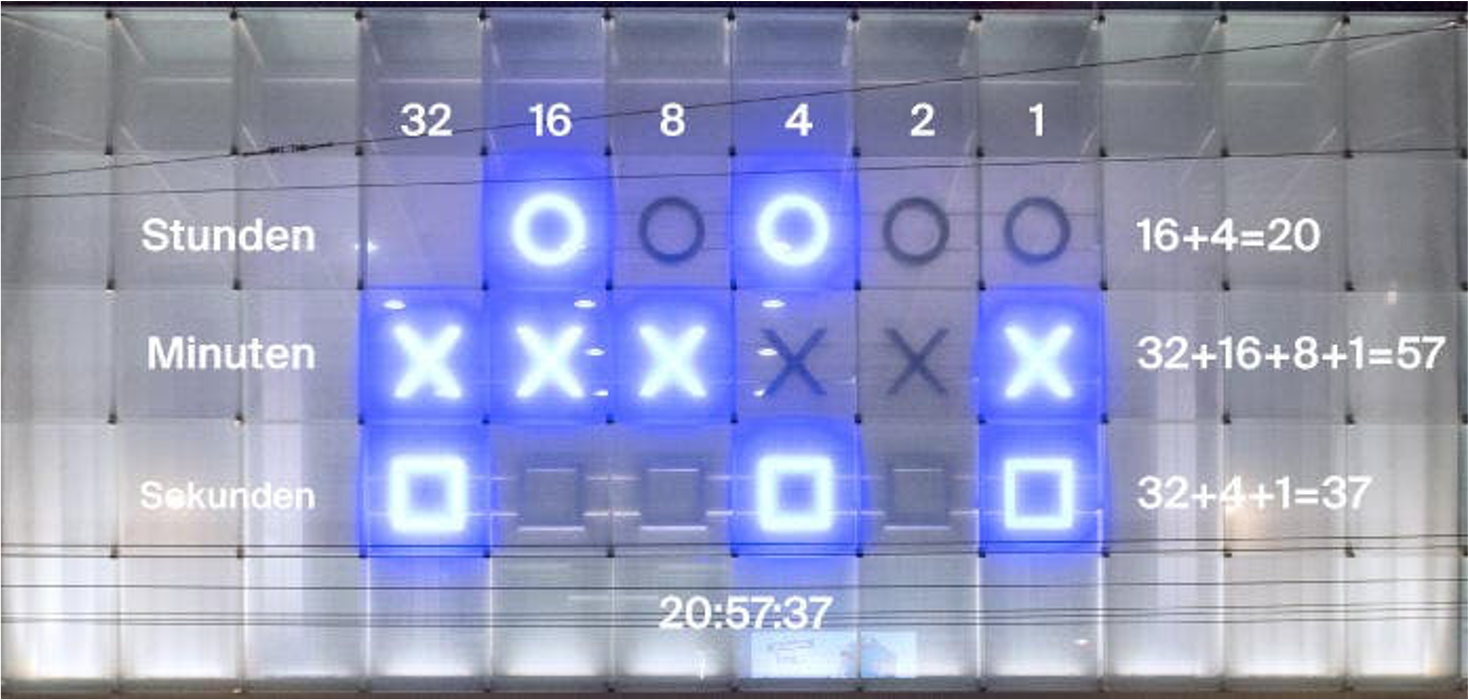
\includegraphics[width=0.9\textwidth]{binary_clock_read_help}
    \end{figure}
\end{frame}

\begin{frame}
    \frametitle{Warm-Up I}
    Uhrzeit 2:
    \begin{figure}[H]
        \centering
        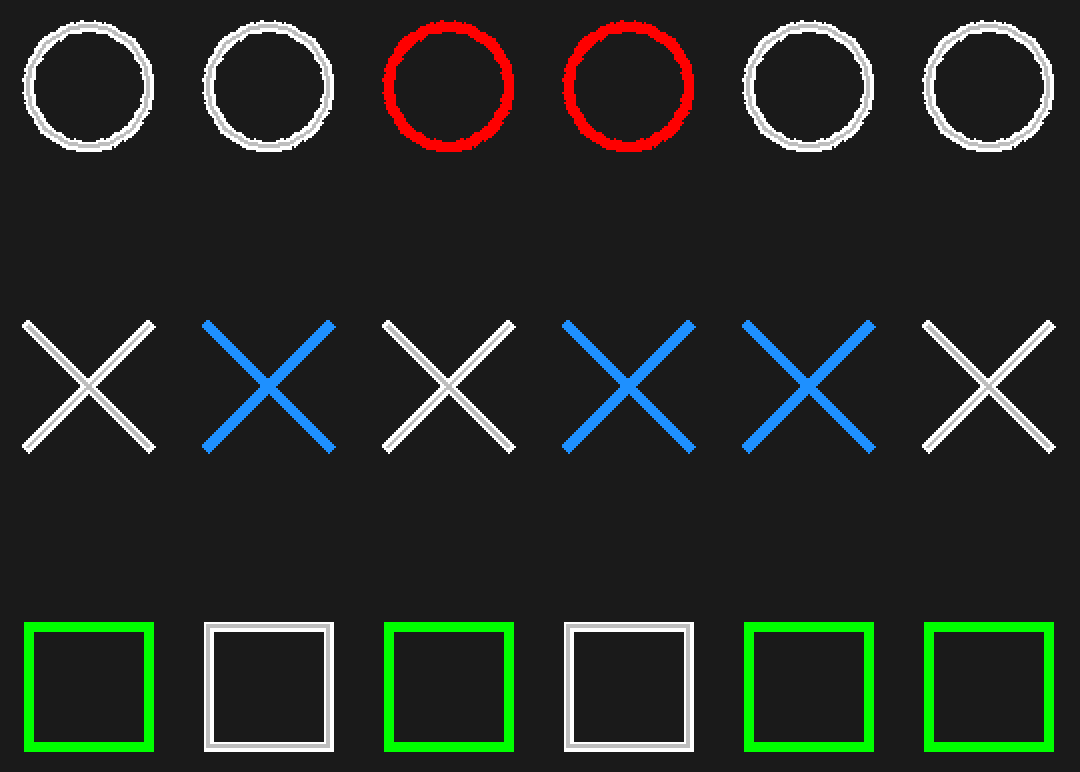
\includegraphics[width=0.7\textwidth]{12_22_43_dark}
    \end{figure}
    \onslide<2-> $$12:22:43$$
\end{frame}

\begin{frame}
    \frametitle{Warm-Up II}
    Frage: Wie weit kann man mit einer Hand zählen?
    \onslide<2->
    \begin{figure}[H]
        \centering
        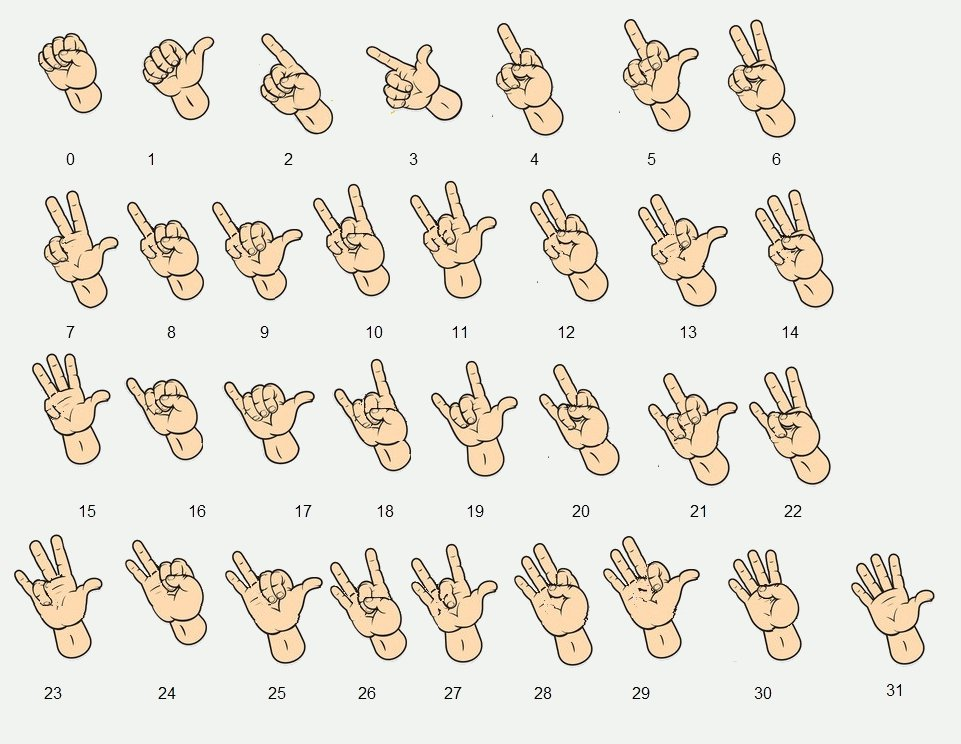
\includegraphics[width=0.7\textwidth]{binarycount}
    \end{figure}
\end{frame}

\begin{frame}
    \frametitle{Ziele}
    \begin{itemize}
        \item Wissen, was ein Zahlensystem ist
        \item \onslide<2-> Wissen, wie Dezimal \& Binärsystem aufgebaut sind
        \item \onslide<3-> Umrechnen Binärsystem $\rightarrow$ Dezimalsystem
        \item \onslide<4-> Code für Umrechnung schreiben
        % \item \onslide<4-> 
    \end{itemize}
\end{frame}

\begin{frame}
    \frametitle{Zahlensysteme}    
    \begin{definition}
        Ein \textbf{Zahlensystem} ist ein System, mit dem Zahlen dargestellt werden. Es wird durch seine \textbf{Basis} und seine \textbf{Nennwerte} festgelegt.
        \linebreak
        \linebreak
        Beispiele für Zahlensysteme sind das uns sehr vertraute Dezimalsystem, das Binärsystem (Basis $2$) oder das Hexadezimalsystem (Basis $16$).
    \end{definition}
\end{frame}

\begin{frame}
    \frametitle{Dezimalsystem}

    \begin{itemize}
        \item Das \textbf{Dezimalsystem} (auch \textbf{Zehnersystem}) ist das Zahlensystem mit \ldots
        \item \onslide<2-> Basis $10$ und \ldots
        \item \onslide<3-> Nennwerte $0,1,2,3,4,5,6,7,8,9$.
        \item \onslide<4-> Die Zahl $1903_{10}$ ist dann wie folgt zu interpretieren:
        \onslide<5->
        \begin{align*}
            \label{equ dezimalzahl in basis und nennwerten}
            \textcolor{blue}{1903}_{\textcolor{magenta}{10}}
            = \textcolor{blue}{1}\times \textcolor{magenta}{10}^{\textcolor{red}{3}} 
            + \textcolor{blue}{9}\times \textcolor{magenta}{10}^{\textcolor{red}{2}} 
            + \textcolor{blue}{0}\times \textcolor{magenta}{10}^{\textcolor{red}{1}} 
            + \textcolor{blue}{3}\times \textcolor{magenta}{10}^{\textcolor{red}{0}}
        \end{align*}
        \item \onslide<6-> Mit der \textit{kleinen Zahl unten rechts} ($\textcolor{magenta}{10}$) deuten wir an, dass die Zahl im Dezimalsystem zu betrachten ist. 
        \item \onslide<7-> Lässt man diese Zahl weg, schreibt man also z.B. $576$, so bedeutet dies (meistens), dass die Zahl im Dezimalsystem steht.
    \end{itemize}
\end{frame}

\begin{frame}
    \frametitle{Binärsystem}

    \begin{center}
        ``\textit{I told my friend 10 jokes about the binary system - He didn't get either of them!}''	
    \end{center}

    \onslide<2-> 

    \begin{definition}
        Die kleinste Informationseinheit ist das \textbf{Bit}, es hat zwei Möglichkeiten: es kann entweder $0$ oder $1$ sein.
        In der Welt der Elektrotechnik hat diese eine besondere Relevanz, da diese den beiden Zuständen `es fliesst kein Strom ($0$)' oder `es fliesst Strom ($1$)' entsprechen. 
        \onslide<3-> 
        \newline
        \newline
        Deshalb ist da das \textbf{Binärsystem} wichtig: Die Basis ist $2$ und die Nennwerte sind $0$ und $1$. Eine Binärzahl besteht also aus mehreren Bits.
    \end{definition}
\end{frame}

\begin{frame}
    \frametitle{Binärsystem}

    Das \textbf{Umrechnen einer Binärzahl in eine Dezimalzahl} geht ganz einfach. Für die Zahl $100101_2$ geht man wie folgt vor:
    \begin{align*}\begin{split}
        \textcolor{blue}{100101}_{\textcolor{magenta}{2}}
        &= \textcolor{blue}{1} \times \textcolor{magenta}{2}^{\textcolor{red}{5}}
        + \textcolor{blue}{0} \times \textcolor{magenta}{2}^{\textcolor{red}{4}}
        + \textcolor{blue}{0} \times \textcolor{magenta}{2}^{\textcolor{red}{3}}
        + \textcolor{blue}{1} \times \textcolor{magenta}{2}^{\textcolor{red}{2}}
        + \textcolor{blue}{0} \times \textcolor{magenta}{2}^{\textcolor{red}{1}}
        + \textcolor{blue}{1} \times \textcolor{magenta}{2}^{\textcolor{red}{0}}
        \\
        &= 32_{10} + 4_{10} + 1_{10}
        \\
        &= 37_{10}		
    \end{split}\end{align*}
\end{frame}

\begin{frame}
    \frametitle{Aufgaben lösen}
    Dossier auf OneNote (beinhaltet alle Theorie von heute)
    \begin{itemize}
        \item Aufgabe 2.1
        \item Aufgabe 3.1
        \item Aufgabe 3.2
        \item Aufgabe 3.3
        \begin{itemize}
            \vspace{-\topsep}
            \item Code: Binärzahl in Dezimalzahl
            \item alleine oder in 2er-Gruppe (keine 3er usw.)
            \item \textcolor{red}{Abgabe bis heute Abend per Teams}
            \item falls in Gruppe gearbeitet nur $1$ Abgabe
            \item keinen kopierten Code abgeben
        \end{itemize}
        
    \end{itemize}
\end{frame}

% \begin{frame}
%     \frametitle{}
%     \begin{itemize}
%         \item 
%         \item \onslide<2-> 
%         \item \onslide<3-> 
%         \item \onslide<4-> 
%     \end{itemize}
% \end{frame}

\end{document}
